% This is LLNCS.DEM the demonstration file of
% the LaTeX macro package from Springer-Verlag
% for Lecture Notes in Computer Science,
% version 2.4 for LaTeX2e as of 16. April 2010
\documentclass{llncs}

\usepackage[cmex10]{amsmath}
\usepackage{amssymb, amsfonts}

\usepackage{natbib}
\usepackage{array,multirow}
\usepackage{color, colortbl}
\usepackage{makeidx}  
\usepackage{rotating}
\usepackage{graphicx}

\definecolor{col1}{rgb}{0.988,0.839,0.571}
\definecolor{col2}{rgb}{0.886,0.886,0.555}
\definecolor{col3}{rgb}{0.582,0.661,0.976}
\definecolor{white}{rgb}{1,1,1}

\graphicspath{{./Figures/},{./Figures/OasisCor/},{./Figures/OasisRegression/},{./Figures/Ellipse/}}
\DeclareGraphicsExtensions{.pdf,.png}



\newcommand{\cost}[0]{\mathtt{c}}
\newcommand{\couplingcost}[0]{\mathtt{cost}}
\newcommand{\coupling}[0]{\pi}
\newcommand{\couplings}[0]{\mathcal{C}}
\def\argmin{\mathop{\rm argmin}}
\newcommand{\dimX}{\mathtt{d}}
\newcommand{\Xsp}{{\mathbf{X}}}
\newcommand{\Ysp}{{\mathbf{Y}}}
\newcommand{\lambdaX}{\lambda^\Xsp}
\newcommand{\lambdaY}{\lambda^\Ysp}
\newcommand{\Cjk}{C_{j,k}}
\newcommand{\CjkX}{C^\Xsp_{j,k}}
\newcommand{\CjkY}{C^\Ysp_{j,k}}
\newcommand{\psijkX}{\psi^\Xsp_{j,k}}
\newcommand{\psijkY}{\psi^\Ysp_{j,k}}




\begin{document}

\title{Exploratory Population Analysis with Unbalanced Optimal Transport}
\titlerunning{Exploratory Population Analysis with Unbalanced Optimal Transport}  

\author{***, ***, ***, ***, ***}%Samuel Gerber, Marc Niethammer, Martin Styner, Stephen Aylward}
\authorrunning{***}%Gerber et al.} 
\institute{***\\%Kitware Inc, Carborro NC 27510, USA,\\
\email{***@***.**}%samuel.gerber@kitware.com}
\and
***%University of North Carolina, Chapel Hill NC 27504, USA}
}

\maketitle              

% What problems are we addressing?
%  - [MRI] disentangle mass from shape changes
%  - [MRI] No segmentations needed
%  - [VESSELS] unstructured point clouds
%  - [VESSELS] background blood perfusion

% What's new?
%  - Hypothesis generation
%  - Different measure to capture changes
%  - No deformable registration
%  - No parameter tuning
%  - [MRI] Unbalanced mass transport
%  - [VESSELS] Decomposition of transport plan with respect to underlying measure


\begin{abstract}
The plethora of data from neuroimaging studies provide a rich opportunity to
discover effects and generate hypotheses through exploratory data analysis. The
pathologies in brain disease often manifest in changes in shape along with
deterioration and alteration of brain matter, i.e., changes in mass. We propose
to use unbalanced optimal transport to disentangle shape from mass changes and
localize those changes. The exploratory analysis approach generates images of
transport cost and mass changes for each subject in the population.  Using
voxelwise correlations with disease indicators on these images highlight
regions of mass or shape changes related to the disease indicator.  We
demonstrate the method on the white and gray matter segmentations from the
OASIS brain MRI data set, which includes subject ranging from healthy to mild
and moderate dementia. The results corroborate known pathology changes related
to dementia and suggest avenues for further clinical research. Additionally
regression and permutation testing on the transport cost and mass change images
improve on existing methods to predict disease measures and indicates that the
proposed method captures a larger portion of pathology induced changes.
\end{abstract}



\section{Introduction}
Neurological disease and disorder manifest in subtle and varied changes in
brain anatomy that can be non-local in nature and effect volumetric as well as
shape change. To detect and quantify these changes is a primary goal of
morphometry based population analysis. We propose a novel morphometry approach
based on unbalanced optimal transport that yields voxelwise comparison that
explicitly separates shape from volumetric changes and can take into account
non-local changes. 

Optimal transport, as the name implies, solves the problem of transporting mass
from a probability measure $\mu$ to a probability measure $\nu$, such that the
cost of moving mass from the source $\mu$ to the target $\nu$ is minimized.
Unbalanced optimal transport extends optimal transport to measures that do not
need to have equal mass by adding a mechanism to create and / or destruct mass
into the optimization problem. The solution of the unbalanced optimal transport
yields a transport map, or coupling, that measures how much mass is moved
between source and target locations. We decompose these transport maps to
measure for each subject, at each voxel, mass allocations and costs of mass
transfer. These two measures explicitly separate mass from shape changes and
due to the non-local nature of optimal transport can take into effect global
effects such as relative position of anatomical structure,  as long as they are
not removed during the spatial normalization phase. The method still depends on
a rigid spatial normalization to bring the subjects into a common coordinate
system were voxelwise comparisons are feasible. After the spatial normalization
the optimal transport derived measures do no depend on a template but instead
are based don averaging pairwise transport maps, which will alleviate bias due
to registrations to a single template  in other methods. 

\begin{figure}[b!]
\scriptsize
\centering
\begin{tabular}{c}
\begin{tabular}{c||c}
\begin{tabular}{cc}
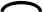
\includegraphics[width=0.1\linewidth]{ellipse0001} &

\includegraphics[width=0.1\linewidth]{ellipse0002} \\
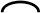
\includegraphics[width=0.1\linewidth]{ellipse0003} &

\includegraphics[width=0.1\linewidth]{ellipse0004} \\
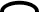
\includegraphics[width=0.1\linewidth]{ellipse0005} &

\includegraphics[width=0.1\linewidth]{ellipse0006} \\
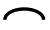
\includegraphics[width=0.1\linewidth]{ellipse0007} &
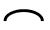
\includegraphics[width=0.1\linewidth]{ellipse0008} \\
%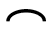
\includegraphics[width=0.1\linewidth]{ellipse0009} & 
%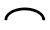
\includegraphics[width=0.1\linewidth]{ellipse0010} \\ 
        \multicolumn{2}{c}{ (a) Data }\\
\end{tabular}
        &
\begin{tabular}{c}
\begin{tabular}{lcr}
\multicolumn{3}{c}{Pearson's r }\\
        -0.9 & 
\includegraphics[width=0.6\linewidth]{colorbar} & 0.9
\end{tabular}\\
\begin{tabular}{l|c|c|c}
%\rowcolor{col3}\\ 
        \hline 
Intensity&
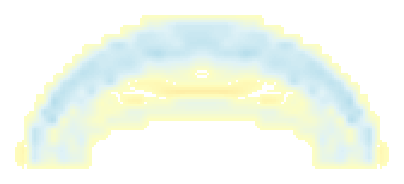
\includegraphics[width=0.18\linewidth]{cor-mass-intensity} &
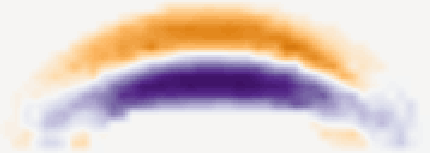
\includegraphics[width=0.18\linewidth]{cor-rx-ry-intensity} &
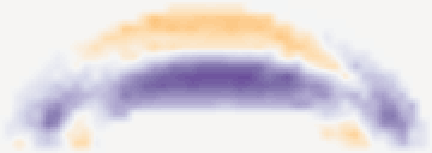
\includegraphics[width=0.18\linewidth]{cor-rx-ry-mass-intensity} \\ \hline
%\rowcolor{col1}
Mass&
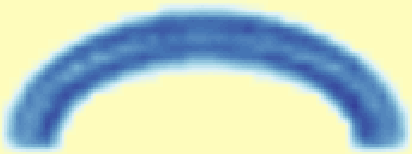
\includegraphics[width=0.18\linewidth]{cor-mass-mass} &
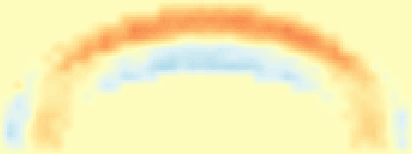
\includegraphics[width=0.18\linewidth]{cor-rx-ry-mass} &
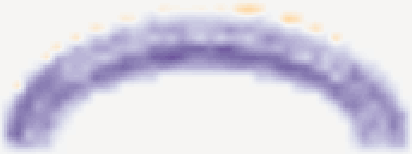
\includegraphics[width=0.18\linewidth]{cor-rx-ry-mass-mass} \\
%\rowcolor{col2}
Cost&
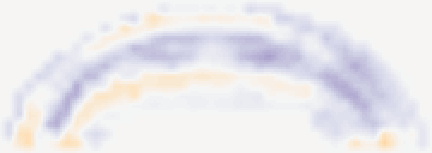
\includegraphics[width=0.18\linewidth]{cor-mass-cost} &
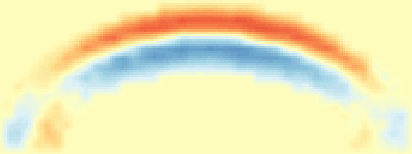
\includegraphics[width=0.18\linewidth]{cor-rx-ry-cost} &
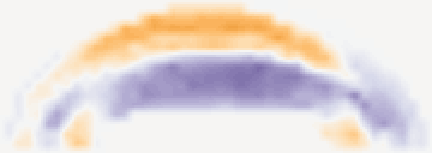
\includegraphics[width=0.18\linewidth]{cor-rx-ry-mass-cost} \\ \hline 
%\rowcolor{white}
        & (b) Size 
        & (c) Shape 
        & (d) Shape + Size 
\end{tabular}
\end{tabular}\\
\end{tabular}
        \\ \hline \hline 
\begin{tabular}{c|c|c}
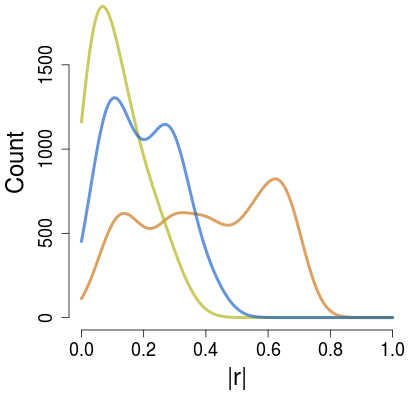
\includegraphics[width=0.3\linewidth]{hist-mass} &
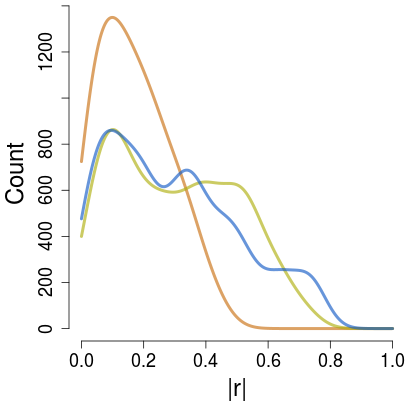
\includegraphics[width=0.3\linewidth]{hist-ellipticity} &
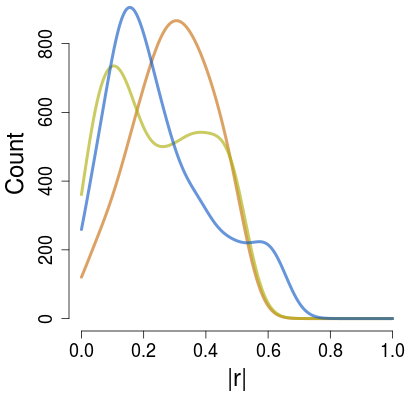
\includegraphics[width=0.3\linewidth]{hist-additive} \\ \hline 
        (e) Size & (f) Shape & (g) Shape + Size
\end{tabular}
\end{tabular}
\caption{\label{fig:cor-ellipse}
Illustration of unbalanced optimal transport on a (a) toy data set of a 100
half ellipses with different minor, major radii and width.  Spatial
correlations of (b) size (number of black pixels), (c) shape (ratio of the
minor and major radii) and (d) sum of size and shape to pixel
intensity values, (middle) mass allocation and (bottom) transport costs.
(f,g,h) Smoothed counts of Pearson's r correlation from the spatial
correlations. The optimal transport approach identifies the changes in size in
the mass imbalance with much stronger correlations than the intensity based
approach.  Shape is captured in both transport cost and intensity, with
slightly stronger correlations with transport cost. Correlation to an additive
shape and mass effect are correctly identified in both transport cost and mass
imbalance, while the intensity values alone lead to weak correlations. The
proposed method correctly identifies shape versus mass effects.  
}
\end{figure}

Figure~\ref{fig:cor-ellipse} illustrates these two optimal transport based
measures on a toy example of a hundred half--ellipses with different
ellipticity and volume.  Correlating the derived measures from the unbalanced
optimal transport solutions with either shape or size of the half--ellipses
shows that the proposed method is capable of correctly attributing changes to
either variation in shape or size.  Traditional voxel-based morphometry does
not indicate the source of the changes and results in weak correlation with
changes in size.

We demonstrate the proposed method on white and gray matter masks of the OASIS
brain data set~\citep{marcus2010open}. We choose to use the gray and white
matter masks instead of MRI intensity values because of the difficulties in
normalizing the intensities across subjects. However, the method can without
modification be applied to continuous graylevel values or with the definition
of a corresponding cost function even to vector or tensor valued measures. The
only requirement is that the measurement are commensurable across subjects.

\section{Related Work}

%Optimal transport and the associated Wasserstein metric, also referred to as
%Earth-movers distance, have been extensively used in computer vision
%applications. Recent advances that permit fast computation of optimal transport
%maps on large data sets lead to a flurry of research in machine learning and 
%Both the mass allocation take into account global effects, in particular the
%shape measures can capture non-local changes, such as
%relative positions of anatomical structures as long as they are no removed
%during the spatial normalization step.  

Voxel-based and tensor-based morphometry (VBM/TBM) are popular approaches to
detect spatially localized anatomical changes~\citep{ashburner2000voxel}. VBM
compares, potentially modulated, intensities at each voxel after
spatial normalization. Similarly TBM compares measures derived, typically the
Jacobian determinant, from a non-linear spatial normalization that aligns the
subjects of the population to a single template at each voxel. 
Voxel-based
morphometry (VBM) yields spatially localized changes in brain anatomy but has
been shown to be sensitive to the particulars of the spatial
normalization~\citep{bookstein2001voxel, davatzikos2004voxel} and has
difficulty in discovering regionally or globally occurring changes. 

Deformation-based morphometry (DBM)~\citep{ashburner1998identifying} adresses
the issue of finding global effects by comparing the parameters of non-linear
spatial normalization to a template.  DBM has successfully been applied for
prediction of pathologies~\citep{gaser2001deformation,lao2004morphological} and been refined to
jointly deal with multiple anatomical
structures~\cite{durrleman2014morphometry} and take into account data dependent
nonlinearity into the estimation of spatial warp
parameters~\citep{gerber2010manifold}. DBM results, typically shown as modes of
variation are more difficult and interpret. Local effects can be teased out of
the spatial warps.

Recent advances in the computation of optimal transport
plans~\citep{cuturi2013sinkhorn,gerber2017multiscale} paved the way for a
flurry in machine learning and applications to medical image
analysis~\citep{cuturi2014fast,gramfort2015fast,rolet2018blind}. In
particular,~\citet{gramfort2015fast} formulate a DBM approach which replaces
non-linear warps by optimal transport maps. 

The unbalanced optimal transport approach presents a different approach to
integrate optimal transport into morphometric analysis. The proposed approach
represents mixture between VBM and DBM methods.  While the results are based
on a voxelwise analysis, the quantities compared stem from a global
optimization problem which can global and regional effects and adds separation
of a effects due to changes in volume from effects due to changes in shape.  A
key observation is that for VBM and TBM the voxelwise measures are driven by
local image gradients and ultimately lead to very similar
results~\citep[Chaper~6]{frackowiak2004human}.  Unbalanced optimal transport
measures solves a global optimization based on the distribution of mass and the
allocation of mass is not driven by the image gradients. Thus, allocation of
mass can be diffuse over a large region without the need for a smooth spatial
normalization to distribute the image gradient driven warp over a larger
region.

%This global optimization  is insensitive to local shifts
%in boundaries since such shifts only incur a small cost of moving mass locally.
%Large cost of moving mass are due to more significant shifts in the anatomy or
%different distributions of mass among different parts of the anatomy. The
%addition of mass allocation with unbalanced optimal transport captures mass
%difference between subject without potentially confounding effects of shape
%changes in non-linear spatial warps. Furthermore 
%VBM

%DBM
%Deformation-based morphometry (DBM) takes a more global approach by analysis of
%deformation fields. While DBM yields overall measures of changes in shape, the
%results are sensitive to the parametrization and regularization of the
%deformation field and require delineation of regions of interest to average
%deformation field statistics. A priori definition of regions defeats the
%purpose of automatic discovery of relevant anatomical changes. 
%Manifold model
%The manifold model approach extends DBM to allow for possible non-linear
%relationships in the data and avoids having to select a template.
%Visualization
%For both approaches visualization of relevant changes is difficult.
%OT map based
%In \cite{} propose an optimal transport based approach that is similar to DBM
%but uses a optimal transport map parametrization to a template. The approach 
%OT voxel based, this work


%Optimal transport is not sensitive to small misalignments in the spatial
%normalization step which result only in a small transport cost of shifting mass
%a short distance. As in VBM the spatial normalization introduces an invariance
%to the spatial affect that are normalized, these can be introduced as in VBM by
%modulating the mass with the Jacobian determinant to correct for volume changes
%otherwise lost in the spatial normalization step. 





\section{Unbalanced Optimal Transport Morphometry}
Morphometry with unbalanced optimal transport follows the standard morphometry
pipeline, but operates on the mass allocation and transport cost maps derived
from the solution of unbalanced optimal transport between the subjects:
\begin{enumerate}
\item Spatial normalization
\item White matter, gray matter and CSF segmentation
\item (optional) Modulation of segmentation by volume changed introduced
through the spatial normalization.
\item {\bf Construct optimal transport mass allocation and cost maps}
\item Smoothing of mass allocation and transport maps
\item Statistical analysis
\end{enumerate}

Section~\ref{sec:unbalanced} describes the unbalanced optimal transport problem
and Section~\ref{sec:mass} the construction of the mass allocation and
transport cost maps for each subject.



\subsection{Unbalanced Optimal Transport}
\label{sec:unbalanced}
For two probability measures  $\mu$ and $\nu$ on probability spaces ${\Xsp}$
and ${\Ysp}$ respectively, a coupling of $\mu$ and $\nu$ is a measure
$\coupling$ on ${\Xsp}\times{\Ysp}$ such that the marginals of $\coupling$ are
$\mu$ and $\nu$. The coupling $\coupling$ defines a {\em transport plan} that
captures how much mass is transport from any $x \in \Xsp$ to  any $y \in \Ysp$
by $\coupling(x, y)$. To define optimal transport and optimal couplings, we
need a cost function $\cost(x,y)$ on ${\Xsp}\times{\Ysp}$ representing the work
or cost needed to move a unit of mass from $x$ to $y$. An optimal coupling
$\coupling^*$ minimizes this cost over all choices of couplings
$\mathcal{C}(\mu,\nu)$ between
$\mu$ and $\nu$: 
\begin{equation}
  \coupling^*= \argmin_{\coupling\in\mathcal{C}(\mu,\nu)} \int_{{\Xsp}}\int_{{\Ysp}}
\cost(x,y)  d\coupling(x,y) \,.  
\end{equation}

For discrete distributions $\mu = \sum_1^n w(x_i) \delta(x_i)$ and $ \nu =
\sum_1^m v(y_i) \delta(y_i)$ with $\sum w(x_i) = \sum v(y_i) = 1$ the optimal
transport problem is equivalent to the linear program 
\begin{equation}
\min_\coupling \sum_{\substack{i=1,\dots,n\\ j=1,\dots,m}} 
      \cost(x_i, y_j) \coupling(x_i, y_j) \quad \text{s.t.}\quad 
\begin{cases}
\sum_j \coupling(x_i, y_j) = \mu(\{x_i\}) = w(x_i) & \\ 
\sum_i \coupling(x_i, y_j) = \nu(\{y_j\}) = v(y_j) & \\
 \coupling(x_i,y_j)\ge 0
\end{cases}\,.
\label{eq:balanced}
\end{equation} 

To extend the formulation to deal with arbitrary positive measures $\mu$ and
$\nu$ which do not sum to one the linear program is modified to allow for the
creation of mass. Define the mass imbalance $\Delta = \sum_1^n v(y_i)  -
\sum_1^m w(x_i)$, the linear program is modified to allow for the creation of
mass at locations $x_i$ by adding a new source location $z$ and target location
and constraints that amount to adding or removing at most $w(x_i)$ to any
location $x_i$ for free. The linear program reads: 
\begin{equation}
\min_\coupling \sum_{\substack{i=1,\dots,n\\ j=1,\dots,m}} 
      \cost(x_i, y_j) \coupling(x_i, y_j) \quad \text{s.t.}\quad 
\begin{cases}
  \sum_j \coupling(x_i, y_j)  = \mu(\{x_i\}) = w(x_i) & \\ 
  \sum_i \coupling(x_i, y_j) + \coupling(z, y_j)= \nu(\{y_j\}) = v(y_j) & \\
  \sum_j \coupling(z, y_j)  = \Delta \\
  \coupling(x_i, y_j) \ge 0 \\
\end{cases}\,.
\label{eq:unbalanced}
\end{equation} 

This modification results in a standard optimal transport problem through the
addition of target location $z$ that can receive or deliver $\Delta$ mass at
zero cost to or from any target location.  Thus, the unbalanced optimal
transport can with only minor modifications be solved by fast approximation
algorithms for large data sets such as the Sinkhorn approach
by~\cite{cuturi2013sinkhorn} or the multiscale strategies
by~\citet{gerber2017multiscale}. 

An arbitrary cost $\cost(z, y_j)$ can be assigned to allocate mass, and $z$
does not need to be restricted to only create or remove $\Delta$ amount of
mass, striking a trade-off between the cost of creating mass and the cost of
moving mass. For our application, we choose the allocation of mass at zero cost
but only allow for the allocation of $\Delta$ mass. This forces all mass in the
target location to be matched to a source location location and distribute the
allocated the mass in such a manner that cost of moving the remaining mass is
minimized.

\subsection{Mass Allocation and Transport Cost Construction}
\label{sec:mass}
To construct the voxelwise mass allocation and transport cost measures we solve
for transport plans $\coupling^*_{i,j}$ between all subjects $X_i$ and $X_j$.  
The variable $z$ in equation~\ref{eq:unbalanced} captures the amount of mass
allocated when moving mass from $X_i$ to $X_j$. Denote by $z_{i, j}$ the mass
allocation variable associated with the optimal transport plan
$\coupling^*_{i,j}$.  By construction $\coupling^*_{i,j}(z_{i,j}, y) =
-\coupling^*_{j,i}(z_{j,i}, x)$ for any $x \in X_i$ and $y \in X_j$.  





\section{Application to OASIS Brain MRI}

The results on the gray matter mask show an increase in the pons area
correlated with CDR and even more so with MMSE.  A hypointense T1 signal in the
pons area has been associated central pontine myelinolysis, which is linked to
alcoholism. The pons in healthy patients typically identified as white matter,
the hypointense signal could potentially lead to a identification with gray
matter, leading to a surplus of gray matter in that area.
\begingroup
\renewcommand{\arraystretch}{0}
\setlength{\tabcolsep}{0pt}
\begin{figure}[tb]
\centering
\begin{tabular}{c}
\begin{tabular}{lcr}
        \multicolumn{3}{c}{\parbox[t][3mm]{20mm}{Pearson's r } }\\
        \parbox[t][3mm]{7mm}{-0.6} & 
        
\includegraphics[width=0.8\linewidth]{colorbar} & 
        \parbox[t][3mm]{6mm}{\hfill 0.6}
\end{tabular}\\
\begin{tabular}{l|cc|cc|cc} 
\parbox[t]{4mm}{\multirow{3}{*}{\rotatebox[origin=c]{90}{Voxel Intensity}}}&
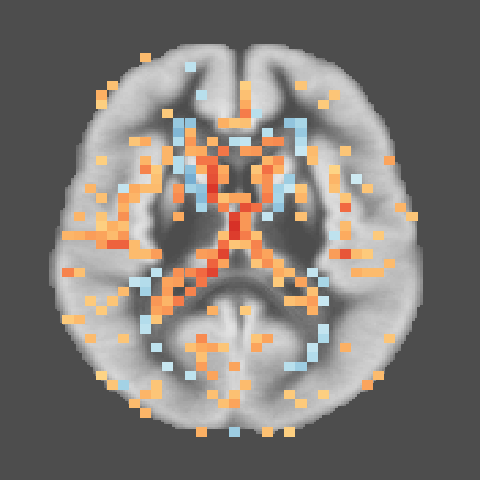
\includegraphics[width=0.14\linewidth]{cor-axial-age-t-iG} &
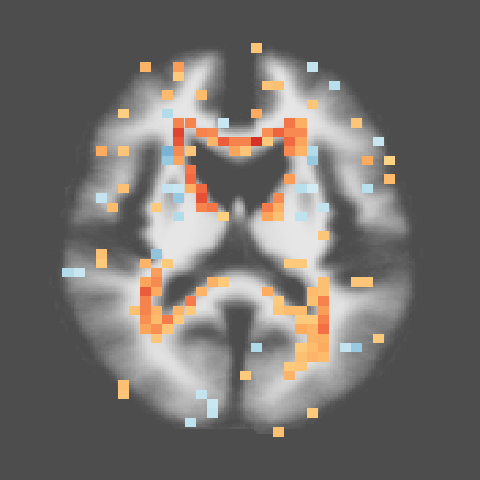
\includegraphics[width=0.14\linewidth]{cor-axial-age-t-iW} &
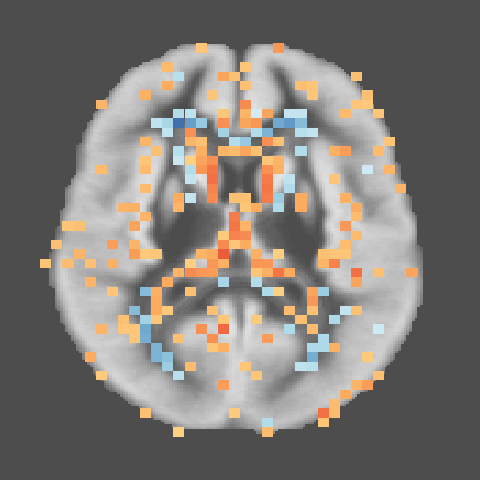
\includegraphics[width=0.14\linewidth]{cor-axial-cdr-t-iG} &
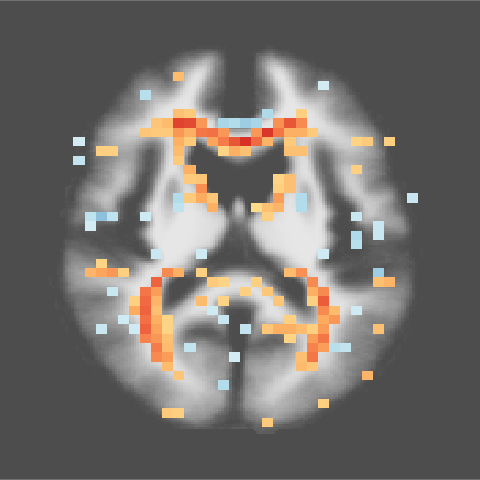
\includegraphics[width=0.14\linewidth]{cor-axial-cdr-t-iW} &
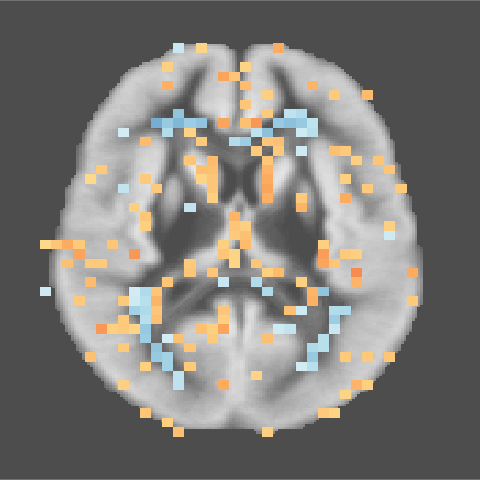
\includegraphics[width=0.14\linewidth]{cor-axial-mmse-t-iG} &
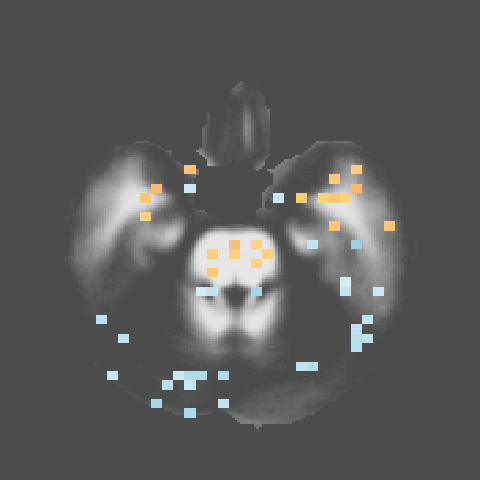
\includegraphics[width=0.14\linewidth]{cor-axial-mmse-t-iW} \\ 
%
        &
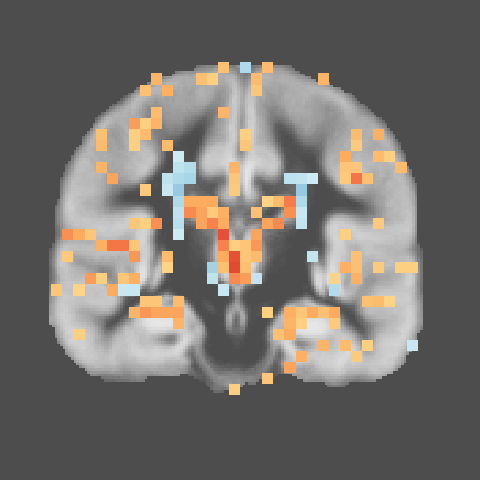
\includegraphics[width=0.14\linewidth]{cor-coronal-age-t-iG} &
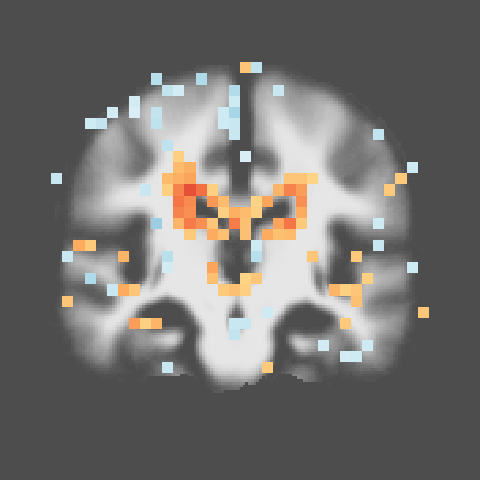
\includegraphics[width=0.14\linewidth]{cor-coronal-age-t-iW} &
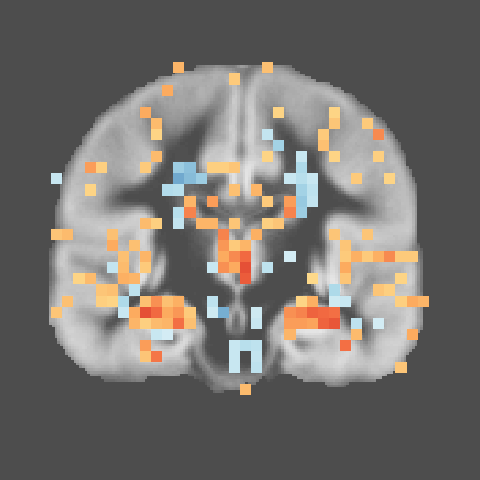
\includegraphics[width=0.14\linewidth]{cor-coronal-cdr-t-iG} &
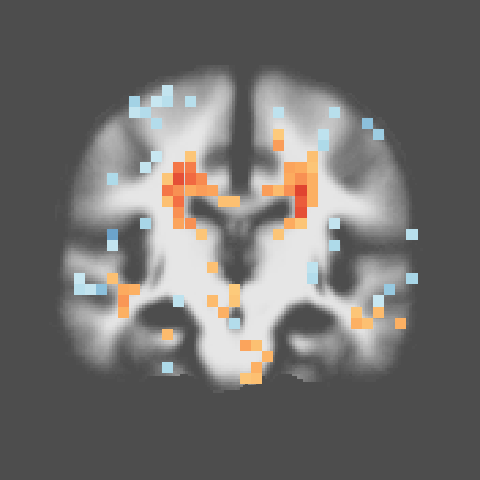
\includegraphics[width=0.14\linewidth]{cor-coronal-cdr-t-iW} &
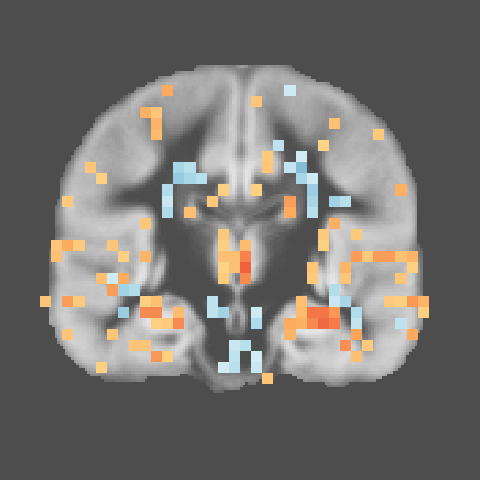
\includegraphics[width=0.14\linewidth]{cor-coronal-mmse-t-iG} &
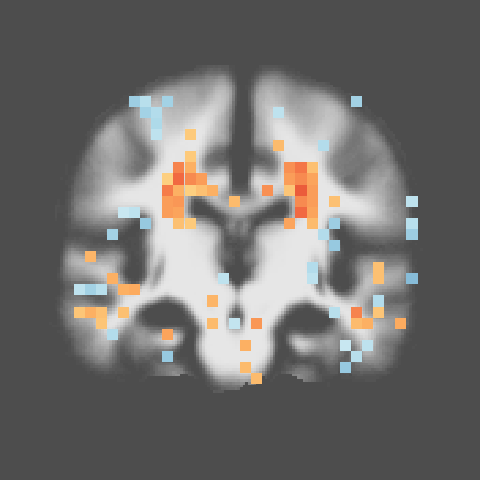
\includegraphics[width=0.14\linewidth]{cor-coronal-mmse-t-iW} \\ 
%
        &
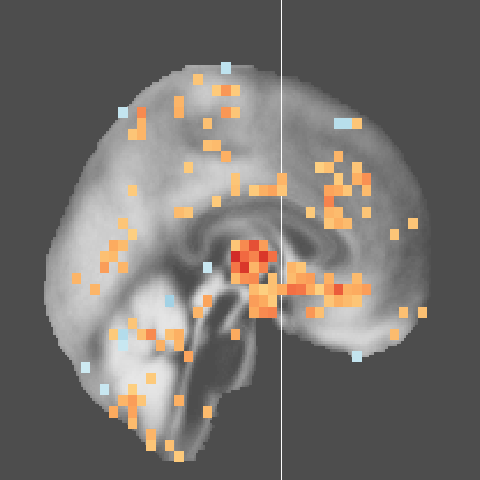
\includegraphics[width=0.14\linewidth]{cor-sagital-age-t-iG} &
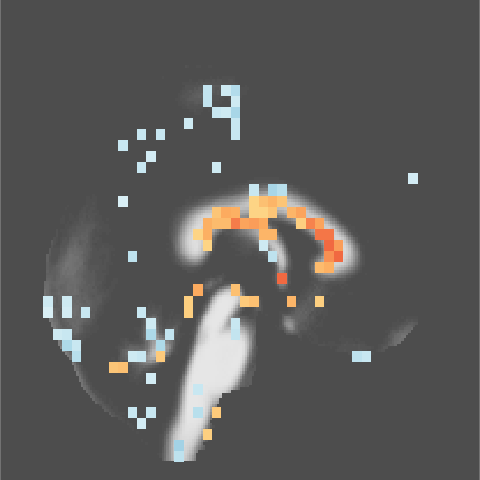
\includegraphics[width=0.14\linewidth]{cor-sagital-age-t-iW} &
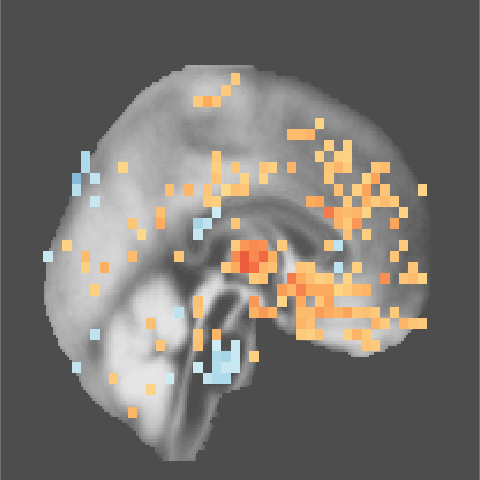
\includegraphics[width=0.14\linewidth]{cor-sagital-cdr-t-iG} &
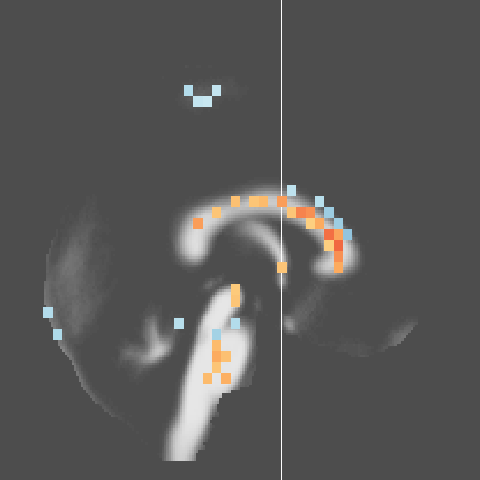
\includegraphics[width=0.14\linewidth]{cor-sagital-cdr-t-iW} &
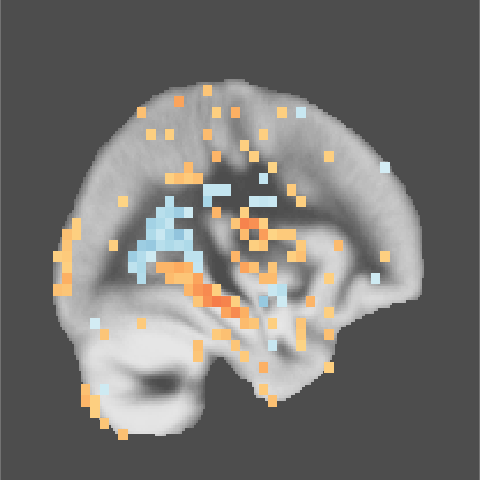
\includegraphics[width=0.14\linewidth]{cor-sagital-mmse-t-iG} &
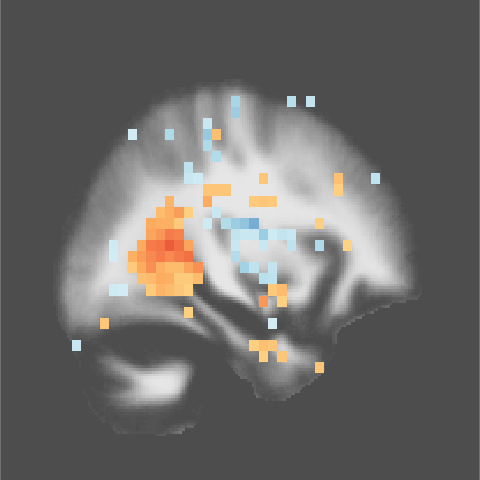
\includegraphics[width=0.14\linewidth]{cor-sagital-mmse-t-iW} \\ \hline \hline
%%
\parbox[t]{4mm}{\multirow{3}{*}{\rotatebox[origin=c]{90}{Mass Imbalance}}}&
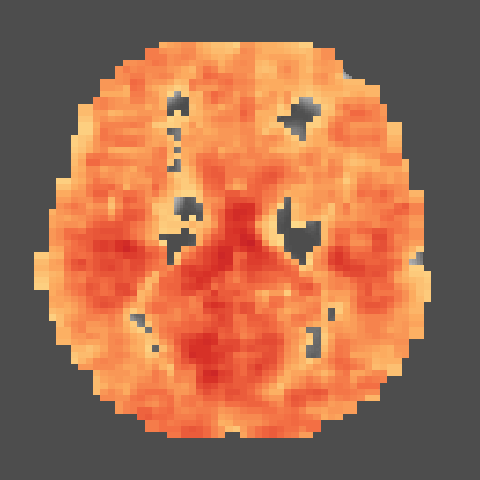
\includegraphics[width=0.14\linewidth]{cor-axial-age-t-mG} &
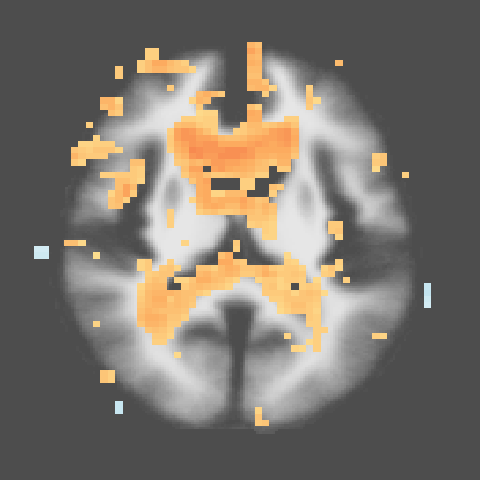
\includegraphics[width=0.14\linewidth]{cor-axial-age-t-mW} &
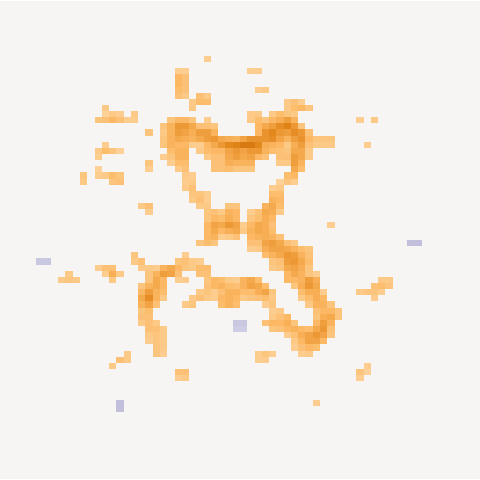
\includegraphics[width=0.14\linewidth]{cor-axial-cdr-t-mG} &
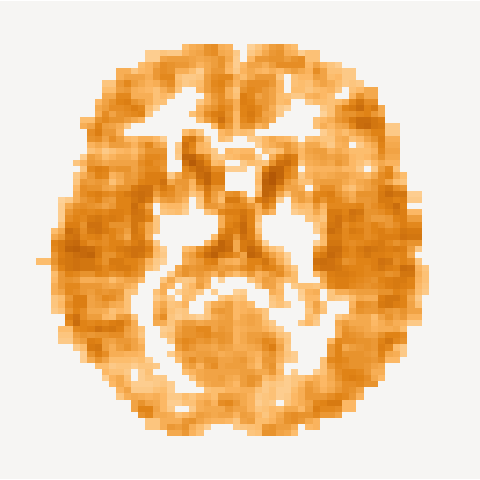
\includegraphics[width=0.14\linewidth]{cor-axial-cdr-t-mW} &
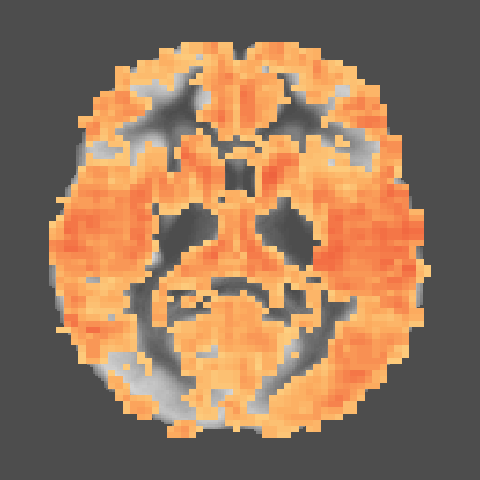
\includegraphics[width=0.14\linewidth]{cor-axial-mmse-t-mG} &
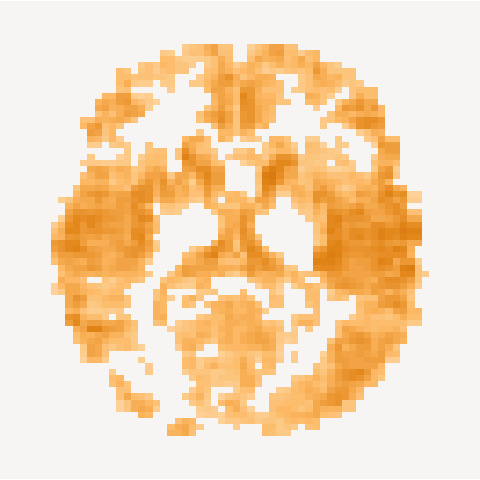
\includegraphics[width=0.14\linewidth]{cor-axial-mmse-t-mW} \\ 
%
        &
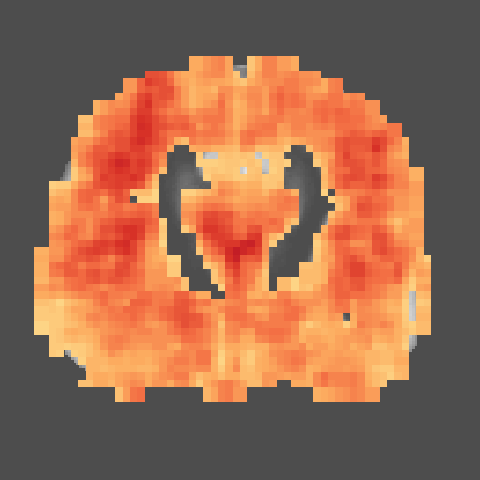
\includegraphics[width=0.14\linewidth]{cor-coronal-age-t-mG} &
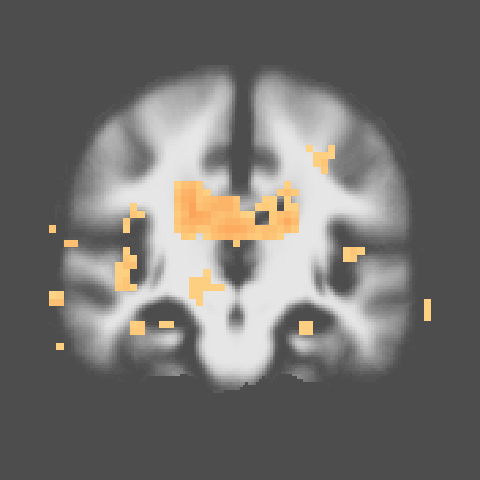
\includegraphics[width=0.14\linewidth]{cor-coronal-age-t-mW} &
\includegraphics[width=0.14\linewidth]{cor-coronal-cdr-t-mG} &
\includegraphics[width=0.14\linewidth]{cor-coronal-cdr-t-mW} &
\includegraphics[width=0.14\linewidth]{cor-coronal-mmse-t-mG} &
\includegraphics[width=0.14\linewidth]{cor-coronal-mmse-t-mW} \\ 
%
        &
\includegraphics[width=0.14\linewidth]{cor-sagital-age-t-mG} &
\includegraphics[width=0.14\linewidth]{cor-sagital-age-t-mW} &
\includegraphics[width=0.14\linewidth]{cor-sagital-cdr-t-mG} &
\includegraphics[width=0.14\linewidth]{cor-sagital-cdr-t-mW} &
\includegraphics[width=0.14\linewidth]{cor-sagital-mmse-t-mG} &
\includegraphics[width=0.14\linewidth]{cor-sagital-mmse-t-mW} \\ \hline \hline
%%
\parbox[t]{2mm}{\multirow{3}{*}{\rotatebox[origin=c]{90}{Transport Cost}}}&
\includegraphics[width=0.14\linewidth]{cor-axial-age-t-tG} &
\includegraphics[width=0.14\linewidth]{cor-axial-age-t-tW} &
\includegraphics[width=0.14\linewidth]{cor-axial-cdr-t-tG} &
\includegraphics[width=0.14\linewidth]{cor-axial-cdr-t-tW} &
\includegraphics[width=0.14\linewidth]{cor-axial-mmse-t-tG} &
\includegraphics[width=0.14\linewidth]{cor-axial-mmse-t-tW} \\ 
%
        &
\includegraphics[width=0.14\linewidth]{cor-coronal-age-t-tG} &
\includegraphics[width=0.14\linewidth]{cor-coronal-age-t-tW} &
\includegraphics[width=0.14\linewidth]{cor-coronal-cdr-t-tG} &
\includegraphics[width=0.14\linewidth]{cor-coronal-cdr-t-tW} &
\includegraphics[width=0.14\linewidth]{cor-coronal-mmse-t-tG} &
\includegraphics[width=0.14\linewidth]{cor-coronal-mmse-t-tW} \\ 
%
        &
\includegraphics[width=0.14\linewidth]{cor-sagital-age-t-tG} &
\includegraphics[width=0.14\linewidth]{cor-sagital-age-t-tW} &
\includegraphics[width=0.14\linewidth]{cor-sagital-cdr-t-tG} &
\includegraphics[width=0.14\linewidth]{cor-sagital-cdr-t-tW} &
\includegraphics[width=0.14\linewidth]{cor-sagital-mmse-t-tG} &
\includegraphics[width=0.14\linewidth]{cor-sagital-mmse-t-tW} \\ \hline \hline
%
& \parbox[b][4mm]{12mm}{Age (w)} 
& \parbox[b][4mm]{12mm}{Age (g)} 
& \parbox[b][4mm]{14mm}{CDR (w)} 
& \parbox[b][4mm]{14mm}{CDR (g) }
& \parbox[b][4mm]{18mm}{MMSE (w)}
& \parbox[b][4mm]{18mm}{MMSE (g)}
\end{tabular}
\end{tabular}
\caption{\label{fig:cor-oasis-gray}
Correlation of Age, MMSE and CDR with smoothed segmentation mask intensity,
optimal transport mass imbalances and optimal transport costs of gray and white
matter.  Correlations are only shown at locations permutation tested p--value
less than 0.05. The background image are average white and gray matter
segmentations. 
} 
\end{figure} \endgroup
A standard VBM analysis is not able to detect the general deterioration for
gray matter related to age, CDR and MMSE.

Figure~\ref{fig:prediction} shows results of fitting elastic nets to the
optimal transport based measures and intensity based measures and comparisons
of linear models of intensity VBM, transport VBM and the global deformation
based approach in~\cite{gerber2010manifold}.  
\begin{figure}[htb]
\scriptsize
\begin{tabular}{cc}
\raisebox{-15mm}{\includegraphics[width=34mm]{glmnet-cvm-permutations}}
        &
\begin{tabular}{l|cccc|cc}
\parbox[2mm]{33mm}{Model}  & 
\parbox[2mm]{11mm}{\centering Residual} & 
\parbox[2mm]{5mm }{\centering $R^2$} & 
\parbox[2mm]{5mm }{\centering F}   & 
\parbox[2mm]{11mm}{\centering p--value}   & 
\parbox[2mm]{7mm }{\centering CVM }  & 
\parbox[2mm]{7mm }{\centering $l_1 R^2$} 
        \\ \hline \hline
\scriptsize
Age, Manifold LDDMM  & 4.4  & 0.14  & 9.9  & 1.0e-4      & NA    & NA  \\
Age, Intensity VBM   & 2.4  & 0.86  & 17.4 & $<\epsilon$ & 4.8   & 0.53  \\
Age, Transport VBM   & 3.1  & 0.74  & 11.1 & $<\epsilon$ & 4.4   & 0.51   \\ \hline
MMSE, Manifold LDDMM & 3.8  & 0.15  & 20.9 & 1.2e-5      & NA    & NA    \\
MMSE, Intensity VBM  & 3.0  & 0.50  &  5.6 & 2.1e-10     & 3.87  & 0.32  \\
MMSE, Transport VBM  & 3.0  & 0.50  & 11.2 & 3.3e-13     & 3.89  & 0.23  \\ \hline
CDR, Manifold LDDMM  & 0.35 & 0.20  & 30.0 & 2.4e-7      & NA    & NA    \\
CDR, Intensity VBM   & 0.19 & 0.79  & 19.5 & $<\epsilon$ & 0.34  & 0.52  \\
CDR, Transport VBM   & 0.26 & 0.61  & 8.5  & 5.2e-15     & 0.34  & 0.36    \\
\end{tabular} \\
        \footnotesize{ (a) } & \footnotesize{ (b) }
\end{tabular}
\caption{ \label{fig:prediction} Prediction with elastic net and comparison to
linear models based on the LDDMM manifold approach.} 
\end{figure}

MMSE  11 nonzeros ( 1tw / 1, 3tg / 3,  7mW / 0 )

CDR 21 nonzeros   ( 3tw / 1, 6tg / 2, 12mw / 0 )

Age 29 nonzeros   ( 4tw / 1, 6tg / 3,  2mg / 1, 17mw / 1 ) 

mmse permuted p-value 0.03, other 0

\section{Conclusion}

Unablanced optimal transport is not restricted to be applied to segmentation
mask, it can be directly applied to graylevel intensities or with an
appropriate cost function to diffusion tensors. 


Combining unbalanced optimal transport with a more globally sensitive analysis.
I.e. the resulting maps are still voxelwise and should be brought into some
correspondence or averaged.

The unbalanced optimal transport forces the creation of mass based on global
mass imbalance between the source and target measures. The approach can be
localized by enforcing regional mass imbalance correction, this might be
sensible to force mass allocation within anatomical corresponding regions and not
allow for redistribution across anatomical different locations. This can be
implement by explicitly adding spatially localized constraint in the same
fashion as the global constrain in equation~\ref{eq:unbalanced}. Alternatively
localization in a more diffuse manner is achieved by adding a cost to
allocation of mass, which effectively will avoid moving mass further than the
allocation penalty since it will be cheaper to create mass in the vicinity.

Additional analysis methods: Clustering

\bibliographystyle{apalike}
\bibliography{bot.bib,optimal-transport}


\end{document}
